\documentclass[a4paper,12pt]{report}
\usepackage[latin1]{inputenc}   % Permet usar tots els accents i car�ters llatins de forma directa.
\usepackage[spanish]{babel}
%\decimalspanish{.}
\usepackage{latexsym}
\usepackage{hyperref}
\usepackage{theorem}
\usepackage{enumerate}
\usepackage{amsfonts, amscd, amsmath, amssymb}
\usepackage[pdftex]{graphicx}
\usepackage{epstopdf}
\usepackage{epsdice}

\setlength{\textheight}{23cm}
\addtolength{\topmargin}{-1.5cm}

\pagestyle{empty}
\begin{document}
\begin{center}
\textbf{\large Estad�stica Aplicada}

\textbf{\large Seguretat i Ci�ncies Policials}

\vskip 0.5 cm
\textbf{\large Activitat dirigida 1}
\end{center}

\vskip 1cm

Volem fer un estudi sobre la classificaci� del RCD Mallorca durant la temporada 2006-07.
Per a aix� disposam de les dades de la seg�ent gr�fica (font LFP):

\begin{center}
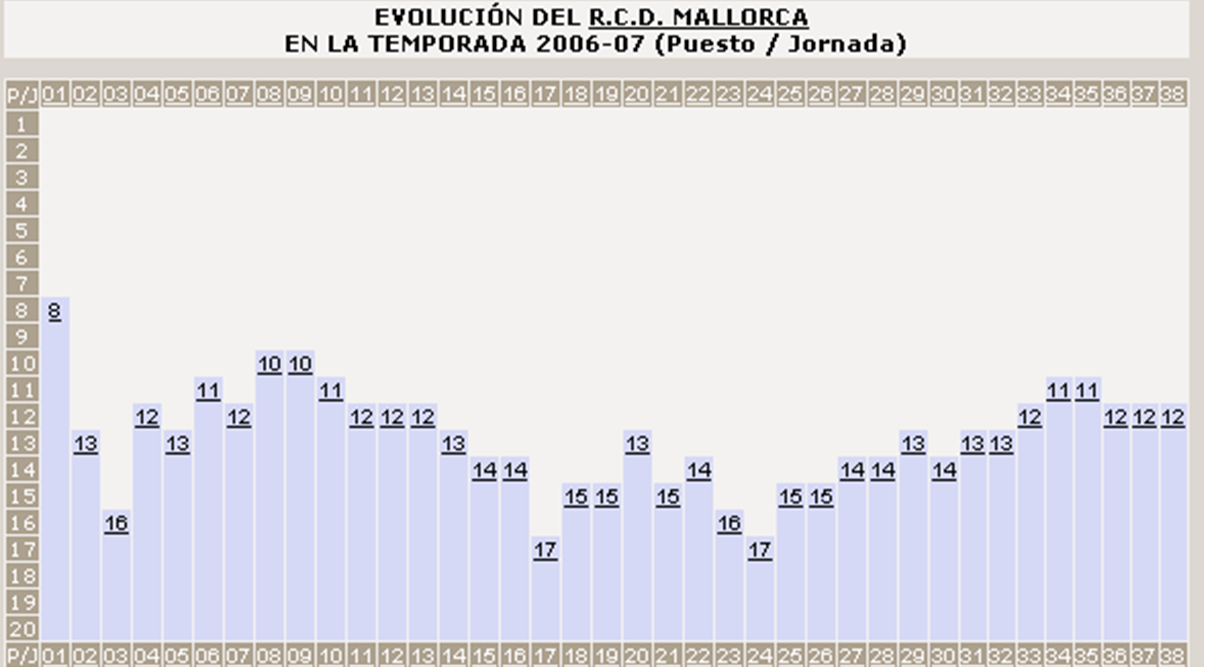
\includegraphics[width=12cm]{rcdmall0607.png}
\end{center}

\begin{enumerate}
\item Quina �s la variable estad�stica que hem d'estudiar? De quin tipus �s?
D�na exemples d'alguns dels seus valors.

\item Construeix la taula de freq��ncies (absolutes, relatives i acumulades en 
cas de que sigui possible) per a la variable considerada.

\item Representa amb un diagrama de barres les freq��ncies absolutes i amb un diagrama
de tarta els percentatges.

\item Quin percentatge de jornades ha estat per davall de la posici� 12? i per damunt de la 15?

\item Calcula la moda.

\item Calcula la mitjana, la mediana, el primer i tercer quartils i el percentil 90 a partir de 
les dades brutes. Fes primer els c�lculs amb la calculadora i despr�s amb la fulla de c�lcul. 

\item Calcula la mitjana, la mediana, el primer i tercer quartils i el percentil 90 a partir de 
les dades de la taula de freq��ncies. Fes primer els c�lculs amb la calculadora i despr�s amb 
la fulla de c�lcul. 

\end{enumerate}


\end{document}